\section{Evaluation}
\label{Section: experiment}

\subsection{Experiment Setup and Configuration Selection}
\label{subsec: configuration}
We carry out real-world experiments on the object detection task (basic computer vision services) to verify our solution’s performance. We use a desktop PC (Intel Xeon E5-2650 v4 CPU) with four NVIDIA 1080ti graphic card as the server infrastructure, and simulate the environment \cite{trade-offs} with three pretrained object detection models in Tensorflow, which are SSD+ResNet152V1, FasterRCNN+ResNet50V1, FasterRCNN+InceptionResNetV2. For each model, two kinds of image resolution, which is $1024\times1024$ and $640\times640$, can be picked up. In our experiment, we set the choices space of fps as \{1, 2, 5, 10, 15, 20, 25, 30\}. We use FFmpeg to switch the frame rate and image resolution, which decide which frames and in what size they should be fed to the object detection model. The configuration space comprises all possible combinations of values of these knobs, so the environment has 48 configurations in total.
%In the service inference, the processing video module uses CPU resources, and the object detection module uses GPU resources. In our study, we use GPU processing time as the metric of resource consumption because GPU is the dominant resource for most video processing workloads \cite{jiang2018chameleon}.In the evaluation, the processing video module needs 62s to decode 5 mins video into 9000 frames image (i.e., average CPU processing time per frame is about 0.006s), which is lower than the GPU processing time. To reduce the latency of processing video, we use different processes to carry out the processing video module and the object detection module in our experiments.   

\subsection{Dataset and Metric}
\label{subsec: datasets}
Most public sources datasets cannot fully satisfy all configuration choices, they provide only a fraction of the requirements for configuration. %for example, some can only guarantee 30 frames but cannot guarantee 1024p resolution. In contrast, others can ensure resolution but cannot provide a sufficient frame rate. 
%In recent years, most of the driving recorder can provide enough resolution and frame rate, so 
We try to search keywords (e.g., ``highway traffic'') on Youtube and download videos that meet the resolution and frame rate requirements. We selecte three datasets: M6, Duke, and Multi-Camera Dataset. M6 is taken from a traffic camera on the longest motorway in Britain. Duke is a video from a fixed camera placed at an intersection, and the traffic flow in the video increases or decreases periodically with the traffic light change. 
%Since the first two datasets were sourced from a fixed camera, 
To ensure that AdaConfigure performs better in multi-camera inference, we combine three videos collected from different locations into one video dataset, Multi-Camera Dataset. The exact content of this dataset varies significantly over time and across space.

For metric, we use the F1 score as the accuracy and average GPU processing time per frame as the resource consumption because GPU is the dominant resource for most video processing workloads \cite{jiang2018chameleon}. F1 score is the harmonic mean of precision and recall, where the precision is true positives divided by the detected objects, and the recall is true positives divided by the ground truth objects. We identify true positives using two conditions, an abounding box-based condition (only check the classified label) and a label-based condition (check the classified label and spatial overlap \cite{overlap}), consistent with prior work \cite{jiang2018chameleon,noscope}. Both accuracy metrics are useful in real video analytics services and used in our experiments. Besides, to compute the accuracy of a frame that is not sampled by exact configuration, we use the location of objects from the previous sampled frame. 
%described in Section \ref{subsec: formulation}.
%, consistent with prior work [24, 32].
%First, to eliminate the bias caused by Cookies and personal preferences, we use private browsing mode to search keywords (e.g., "drivecam highway hd"). Second, manually delete irrelevant videos (e.g., ads for some driving recorders) and download videos that are longer than ten minutes. These videos need to be as dynamic as the real world, such as not standing still for too long. Because none of these videos contained ground truth, we used the original video output data from DNN as the tags to calculate the accuracy. For instance, in object detection, the accuracy is defined by the F1 score with respect to the server-side DNN output in highest resolution (original) with over 50$\%$ confidence score.Based on the above filtering strategy, we finally selected three datasets: 

%we selected three datasets:
%M6: The M6 is the longest motorway in Britain and the most important road from the Midlands to the West Coast. Thousands of cars travel on it every day. This video was taken from a traffic camera, and its natural dynamics allows us to experiment with this video.
%
%Duke: Duke is a video from a fixed camera placed at an intersection. Because it is fixed in the middle of the intersection, the traffic flow in the video increases or decreases periodically as the traffic light change.
%
%Mutli Camera Dataset: Since the first two datasets were sourced from a fixed camera, in order to ensure that AdaConfigure still has better performance when road conditions change dramatically, we used three videos collected from the dashcam, and since they are relatively similar, we combined them into one video.

%\begin{figure*}[!t]
%	\begin{minipage}[t]{0.32\linewidth}
%		\centerline{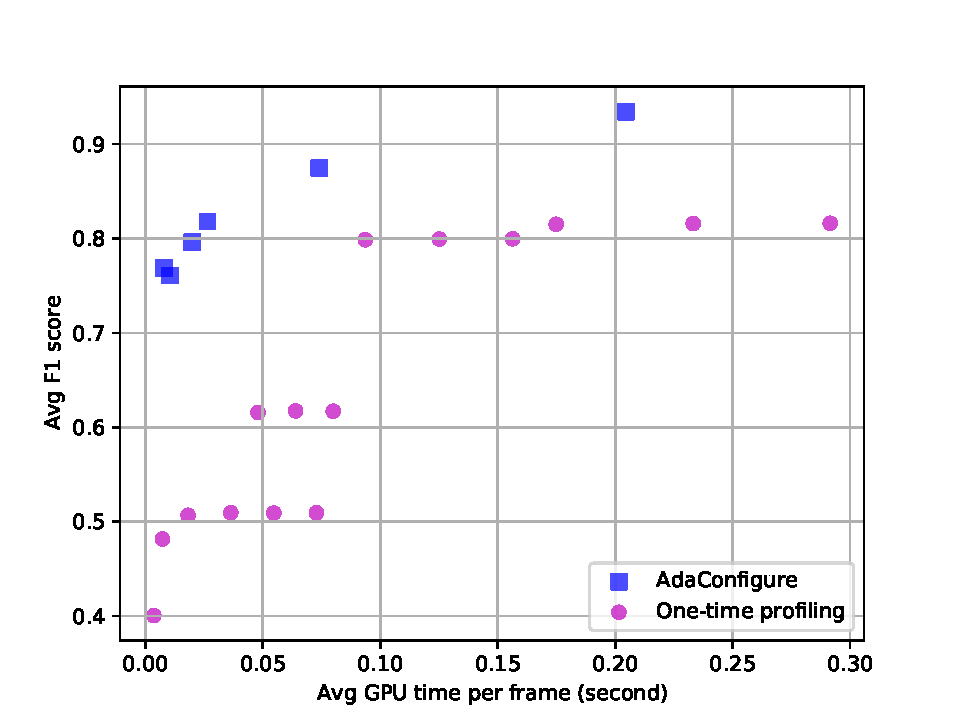
\includegraphics[width=6.5cm]{figures/m6.pdf}}
%		\centerline{(a) M6 (Bounding box-based)}
%	\end{minipage}
%	\hfill
%	\begin{minipage}[t]{0.32\linewidth}
%		\centerline{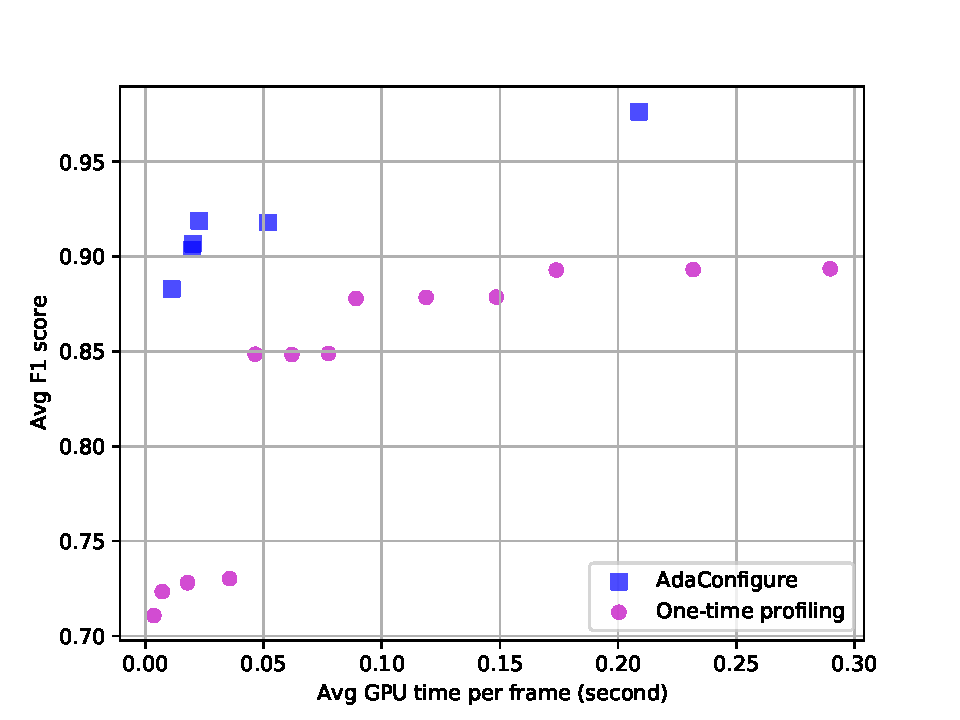
\includegraphics[width=6.5cm]{figures/duke.pdf}}
%		\centerline{(b) Duke (Bounding box-based)}
%	\end{minipage}
%	\hfill
%	\begin{minipage}[t]{0.32\linewidth}
%		\centerline{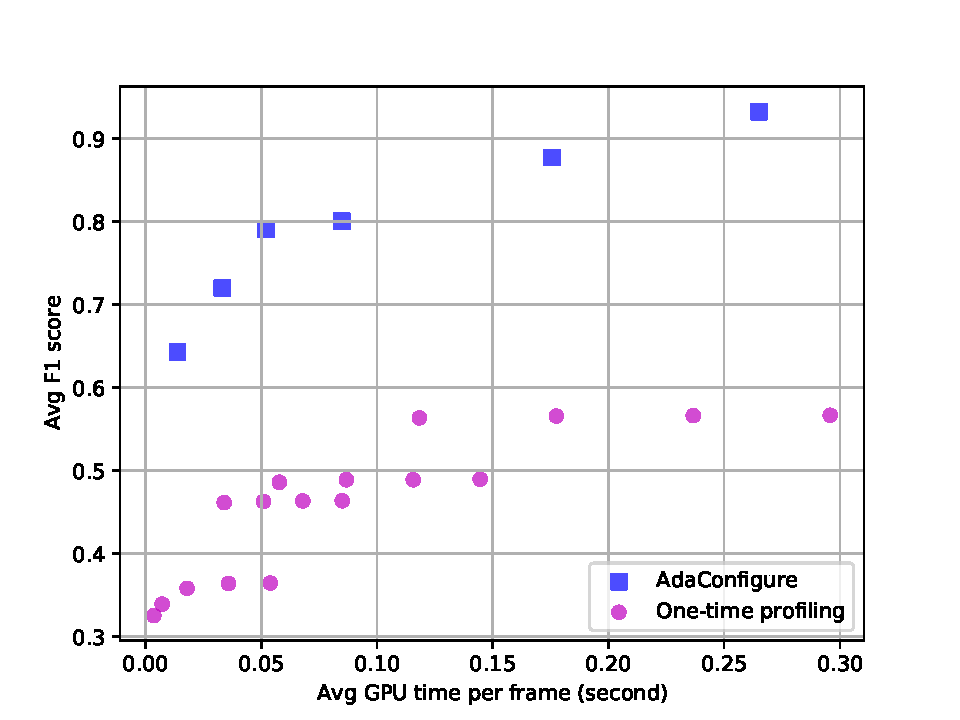
\includegraphics[width=6.5cm]{figures/_Westbound_Eastbound_Rear.pdf}}
%		\centerline{(c) Multi-Camera Dataset (Bounding box-based)}
%	\end{minipage}
%	\vfill
%%	\vspace{0.4cm}
%	\begin{minipage}[t]{0.32\linewidth}
%		\centerline{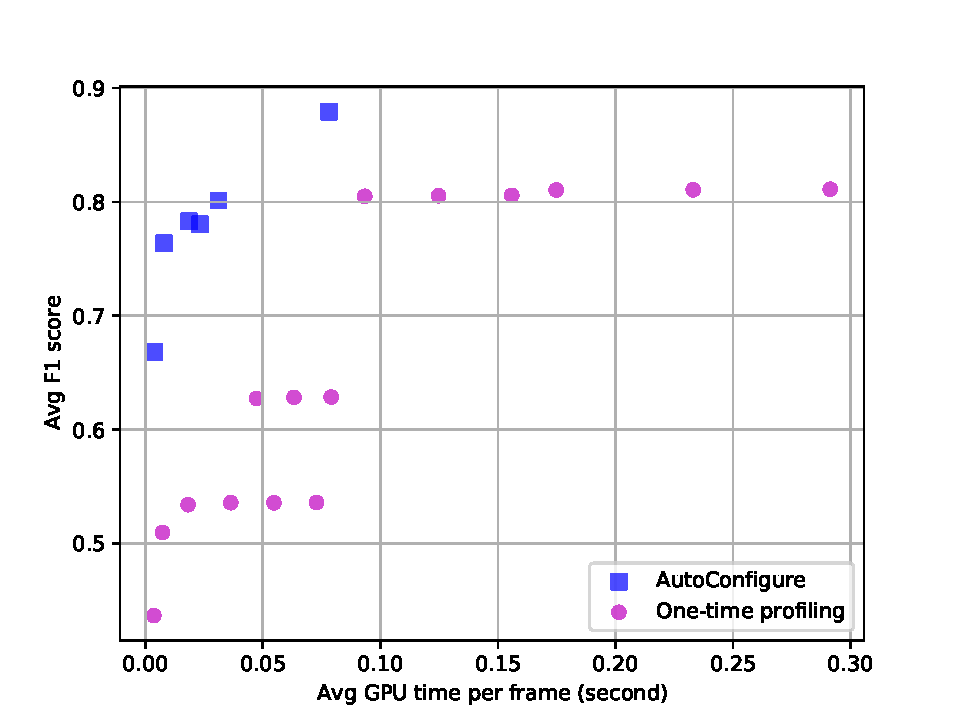
\includegraphics[width=6.5cm]{figures/m6_label.pdf}}
%		\centerline{(d) M6 (label-based)}
%	\end{minipage}
%	\hfill
%	\begin{minipage}[t]{0.32\linewidth}
%		\centerline{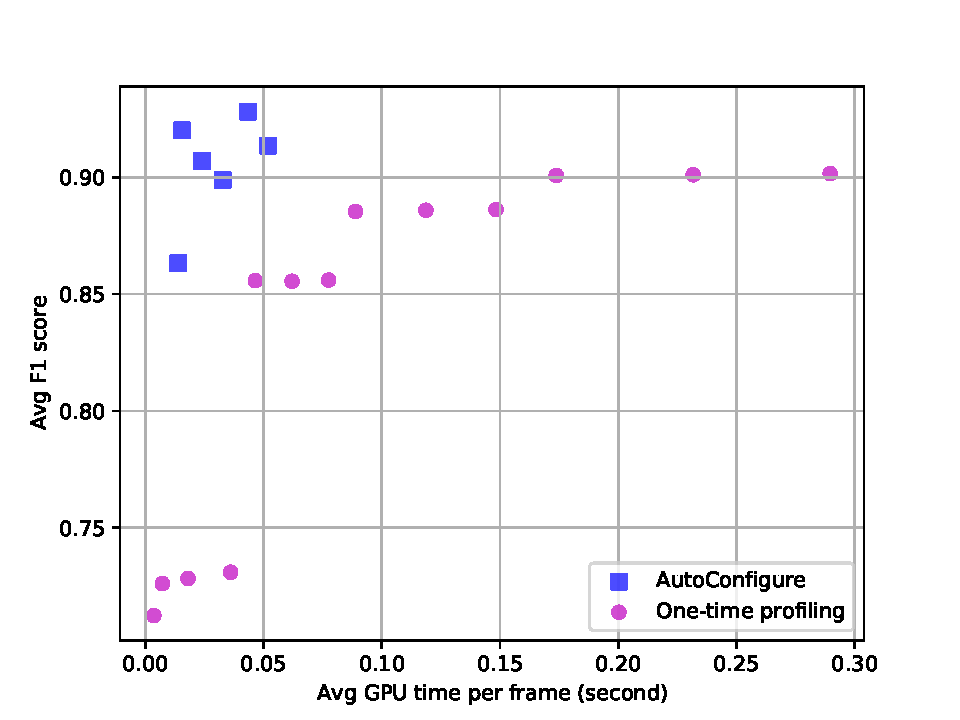
\includegraphics[width=6.5cm]{figures/duke_label.pdf}}
%		\centerline{(e) Duke (label-based)}
%	\end{minipage}
%	\hfill
%	\begin{minipage}[t]{0.32\linewidth}
%		\centerline{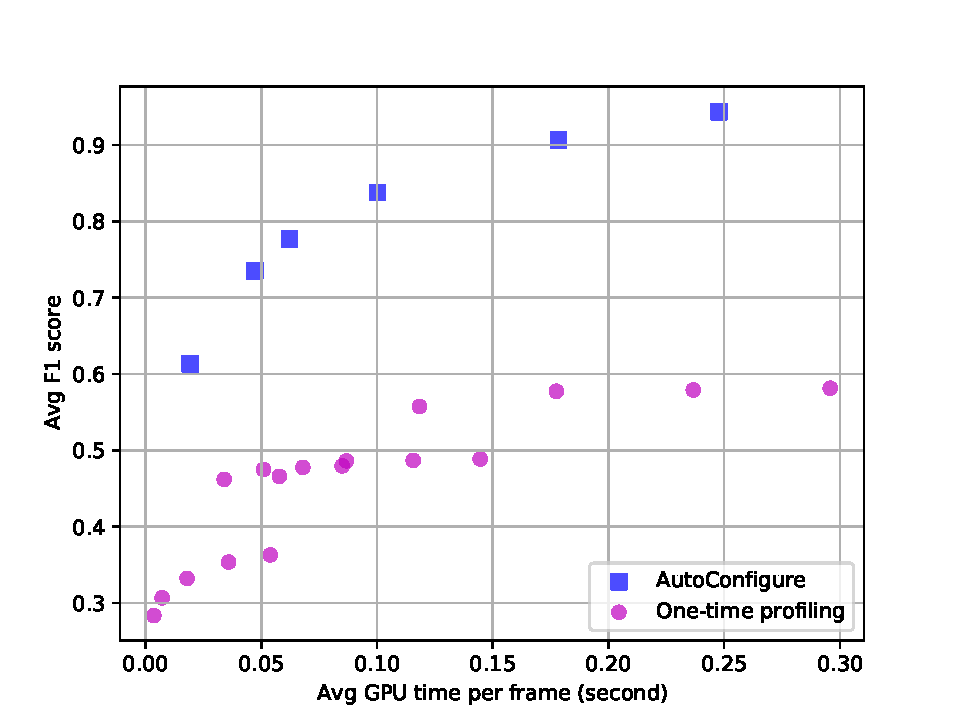
\includegraphics[width=6.5cm]{figures/_Westbound_Eastbound_Rear_label.pdf}}
%		\centerline{(f) Multi-Camera Dataset (label-based)}
%	\end{minipage}		
%	\caption{AdaConfigure (blue) consistently outperforms the baseline of one-time profiling (magenta) across different metrics on different datasets. Each dot represents the results of running each solution.}
%	\label{fig: results}
%\end{figure*}

\begin{figure}[!t]
	\begin{minipage}[t]{0.47\linewidth}
	\centerline{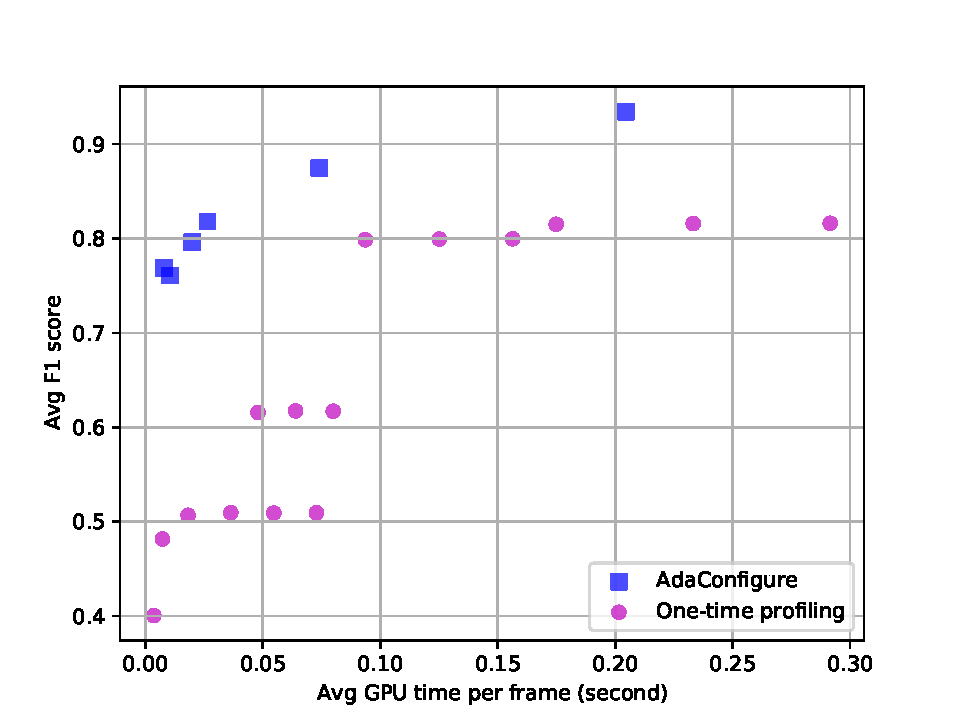
\includegraphics[width=5cm]{figures/m6.pdf}}
	\centerline{(a) M6 (Bounding box-based)}
	\end{minipage}
	\hfill
	\begin{minipage}[t]{0.47\linewidth}
	\centerline{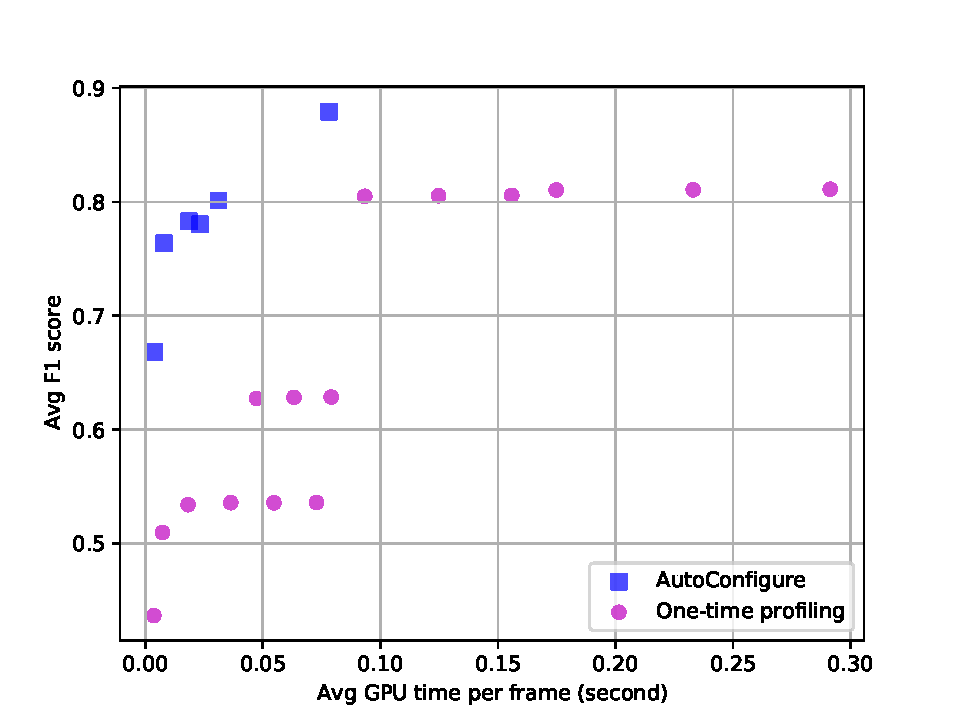
\includegraphics[width=5cm]{figures/m6_label.pdf}}
	\centerline{(b) M6 (label-based)}
	\end{minipage}
	\vfill
	\begin{minipage}[t]{0.47\linewidth}
	\centerline{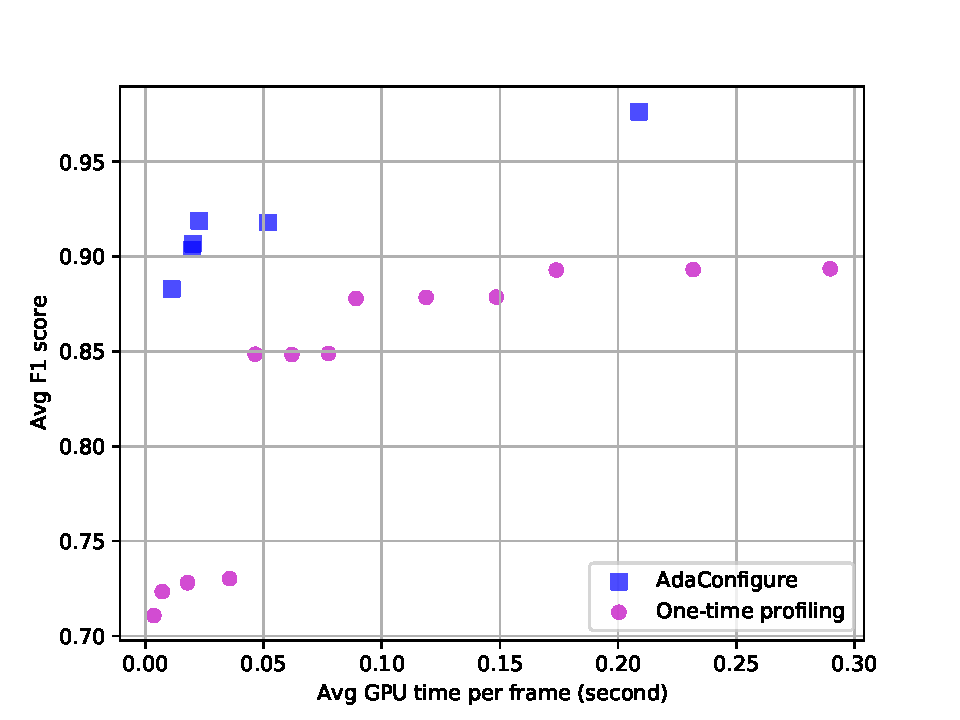
\includegraphics[width=5cm]{figures/duke.pdf}}
	\centerline{(c) Duke (Bounding box-based)}
	\end{minipage}
	\hfill
	%	\vspace{0.4cm}
	\begin{minipage}[t]{0.47\linewidth}
	\centerline{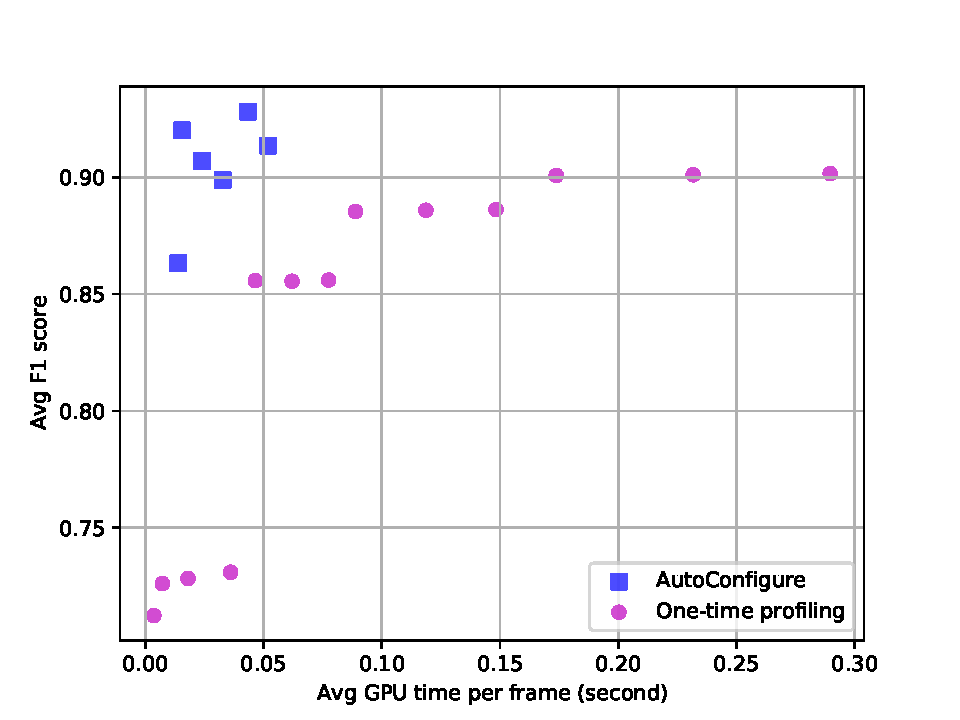
\includegraphics[width=5cm]{figures/duke_label.pdf}}
	\centerline{(d) Duke (label-based)}
	\end{minipage}
	\vfill
	\begin{minipage}[t]{0.47\linewidth}
	\centerline{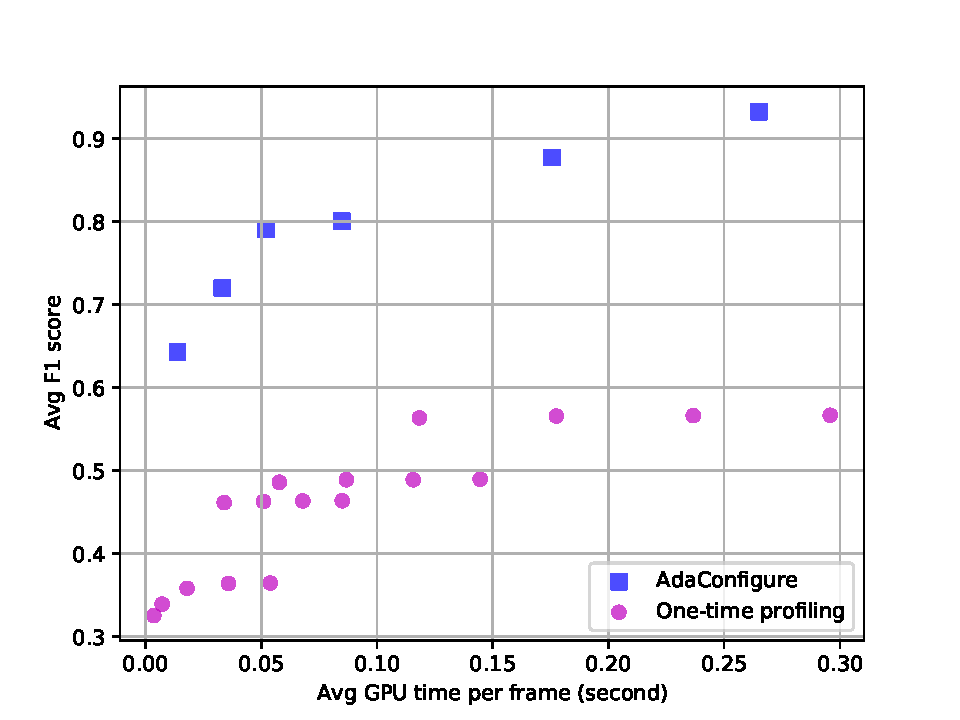
\includegraphics[width=5cm]{figures/_Westbound_Eastbound_Rear.pdf}}
	\centerline{(e) Multi-Camera Dataset }%\\ (Bounding box-based)}
	\centerline{(Bounding box-based)}
	\end{minipage}
	\hfill
	\begin{minipage}[t]{0.47\linewidth}
	\centerline{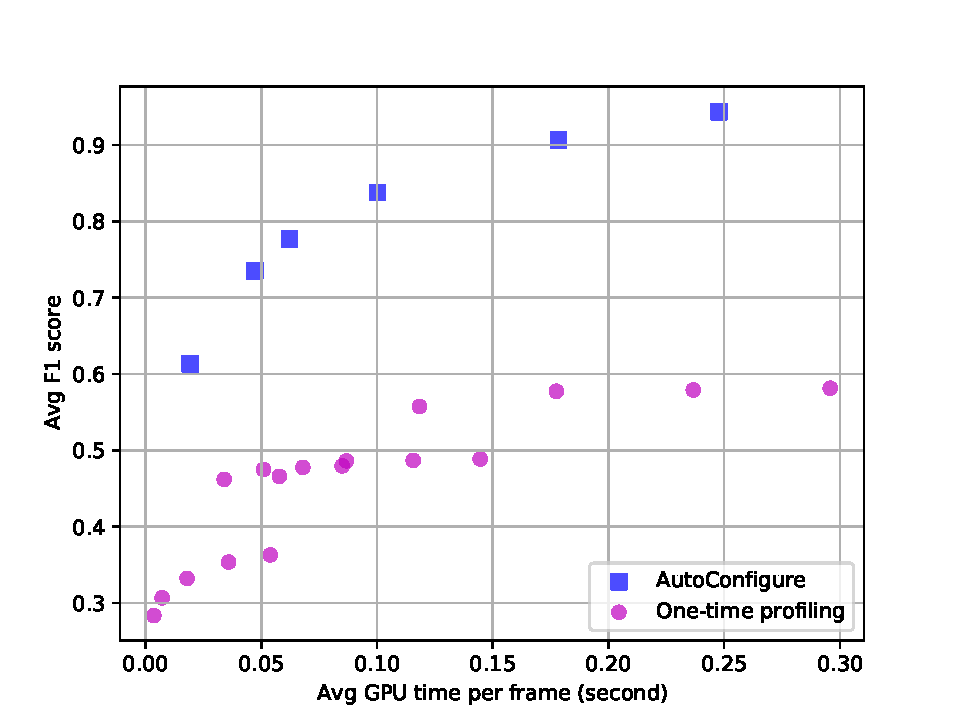
\includegraphics[width=5cm]{figures/_Westbound_Eastbound_Rear_label.pdf}}
	\centerline{(f) Multi-Camera Dataset }% (label-based)}
	\centerline{(label-based)}
	\end{minipage}		
	\caption{AdaConfigure (blue) consistently outperforms the baseline of one-time profiling (magenta) across different metrics on different datasets. Each dot represents the results of running each solution.}
	\label{fig: results}
%	\vspace{-0.5cm} 
\end{figure}

\subsection{Experiment Parameters}
%We apply a deep Q-learning network policy to train the agent. 
In the training procedure, we build up to eight independently identical environments for each data set to speed up the training and decrease the data's dependency. For each dataset, we train the agent 5 epochs and 600 steps (5 mins) per epoch. Some important hyperparameters in our experiments are given in Table ~\ref{tab: parameters}.
%The leaning rate is set to 0.001.

\begin{table}[!t]
	\centering
	%     \begin{tabular}{llllll}
	\resizebox{0.4\textwidth}{!}{
		\begin{tabular}{cccccc}
			\toprule
			Notation          & Value & & & Notation     & Value  \\ \midrule
			$\epsilon$    & 0.8    & & & $k_1$      & 3   \\
			$\gamma$      & 0.9  & & & $k_2$    & 3    \\
			$ \beta $ & 0.2,0.3,...,0.7 & & & $ T (train) $ & 1  \\
			$ t(inference)  $  &  1   & & &   $ T (inference)  $  &  4      \\ 
			\bottomrule
	\end{tabular}}
	\caption{Experiment parameters}
	\label{tab: parameters}
%	\vspace{-0.5cm}
\end{table}

\subsection{Experiment Results}
%We use bounding box-based and label-based metric to evaluate AdaConfigure on M6, Duke, and Multi-Camera Dataset video streams. at the beginning of a video stream \{SSD+ResNet152V1, 640p, 2fps\},
Figure \ref{fig: results} shows that AdaConfigure consistently outperforms the static configuration baseline (only profiling configurations once) along with resource consumption and two accuracy metrics on different datasets. Each magenta dot represents one static configuration solution (one-time profiling).
These static configuration solutions include some fixed expensive configurations and fixed cheap configurations. 
%These static configuration solutions include some expensive configurations, such as \{FasterRCNN+InceptionResNetV2, 640p, 30fps\}, \{FasterRCNN+ResNet50V1, 1024p, 25fps\}, and some cheap configurations, such as \{SSD+ResNet152V1, 640p, 1fps\}, \{SSD+ResNet152V1, 640p, 5fps\}.
Each blue dot represents one AdaConfigure configuration solution, which is dependent on the balance factor $\beta$ in reward function, presented in Section \ref{subsec: reward}. The detailed discussion about different AdaConfigure solutions is in Section \ref{subsec: different sulutions}. Note that AdaConfigure's resource consumption includes both running the best configuration to get inference results and profiling cost of adaptive configuration, which detailed discussed in \ref{subsec: profiling cost}. 

As shown in Figure \ref{fig: results}, Adaconfigure achieves a high accuracy of 10-35\% with the same amount of computing resources, which benefits from the adaptive selection of relatively expensive configuration when the video content is complex (e.g., traffic congestion, high-speed vehicles). Also, Adaconfigure achieves a 50-90\% reduction in resource consumption while achieving almost the same precision as the baseline, which benefits from the adaptive selection of relatively cheap configurations when the video content is simple (e.g., low-traffic flow).

%As shown in Figure \ref{fig: results}, Adaconfigure achieves a high accuracy of 10-35\% with a similar amount of computing resources or achieves a 50-90\% reduction in resource consumption while achieving almost the same precision as the baseline.  

%As shown in Figure \ref{fig: results}, (1) Adaconfigure achieves a high accuracy of 10-35\% with the same amount of computing resources, indicating that it can benefit resource constrained settings (for example, edge or mobile devices). (2) Adaconfigure achieves a 50-90\% reduction in resource consumption while achieving almost the same precision as the baseline, saving capital costs when resources are resilient but expensive (for example, cloud virtual machines).

%As shown in Figure \ref{fig: results}, there are similar results in different datasets.  

%As shown in Figure \ref{fig: results}(a)(b), AdaConfigure achieves 10-30\% higher accuracy with a similar amount of resources, or achieve a similar accuracy with only 20-40\% of the resources on the M6 dataset. As shown in Figure \ref{fig: results}(c)(d), AdaConfigure achieves 10-20\% higher accuracy with a similar amount of resources, or achieve a similar accuracy with only 10-20\% of the resources on a Duke dataset. As shown in Figure \ref{fig: results}(e)(f), AdaConfigure achieves 25-35\% higher accuracy with a similar amount of resources, or achieve higher accuracy with only 15-25\% of the resources on Multi-Camera Dataset. In a word, AdaConfigure can improve 10-35\% higher accuracy or save 60-90\% resource consumption.

%\subsubsection{Superior Performance on Multi-camera Situation}
%\label{subsec: superior performance}
%
%\begin{figure}[!t]
%	\begin{minipage}[t]{0.47\linewidth}
%		\centerline{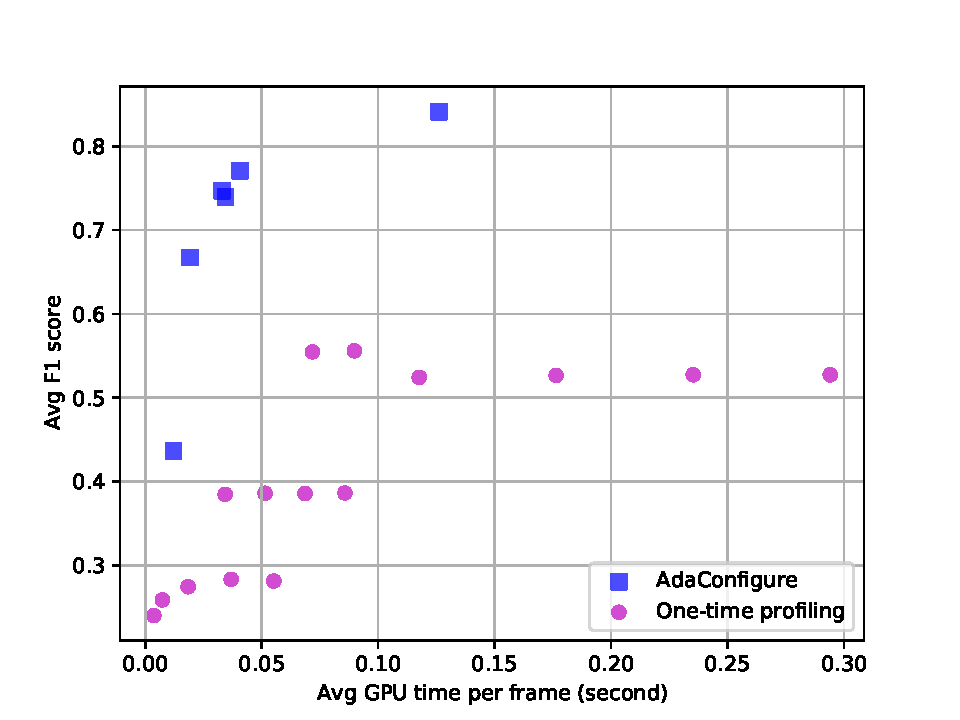
\includegraphics[width=5cm]{figures/Westbound.pdf}}
%		\centerline{(a) Camera 1 }%(Bounding box-based)}
%		\centerline{(Bounding box-based)}
%	\end{minipage}
%	\hfill
%	\begin{minipage}[t]{0.47\linewidth}
%		\centerline{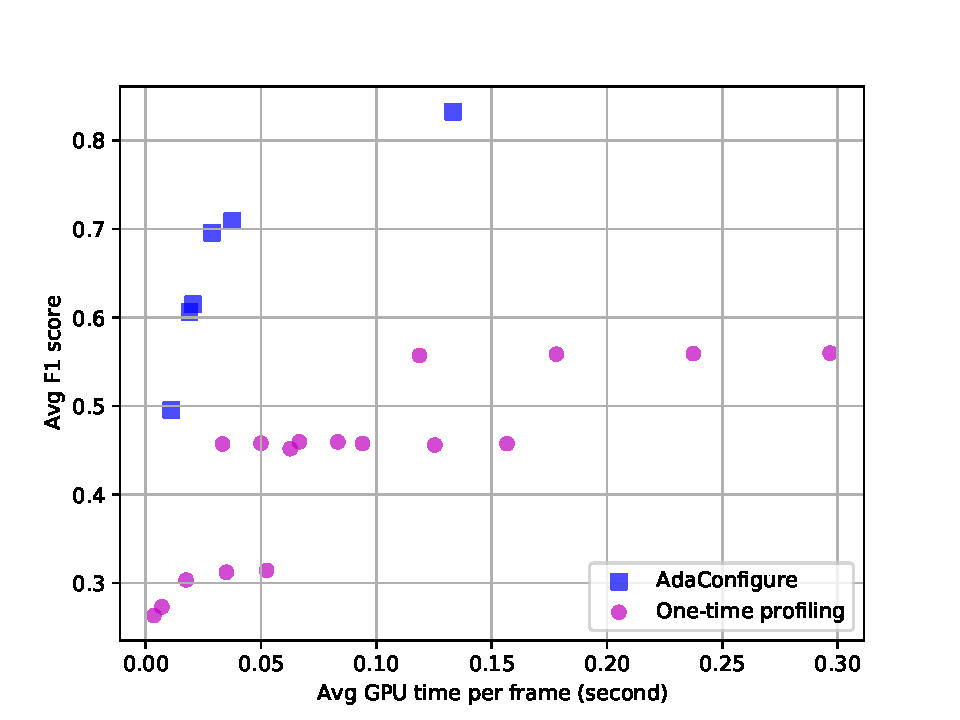
\includegraphics[width=5cm]{figures/Eastbound.pdf}}
%		\centerline{(b) Camera 2 }%(Bounding box-based)}
%		\centerline{(Bounding box-based)}
%	\end{minipage}
%	\vfill
%	\begin{minipage}[t]{\linewidth}
%		\centerline{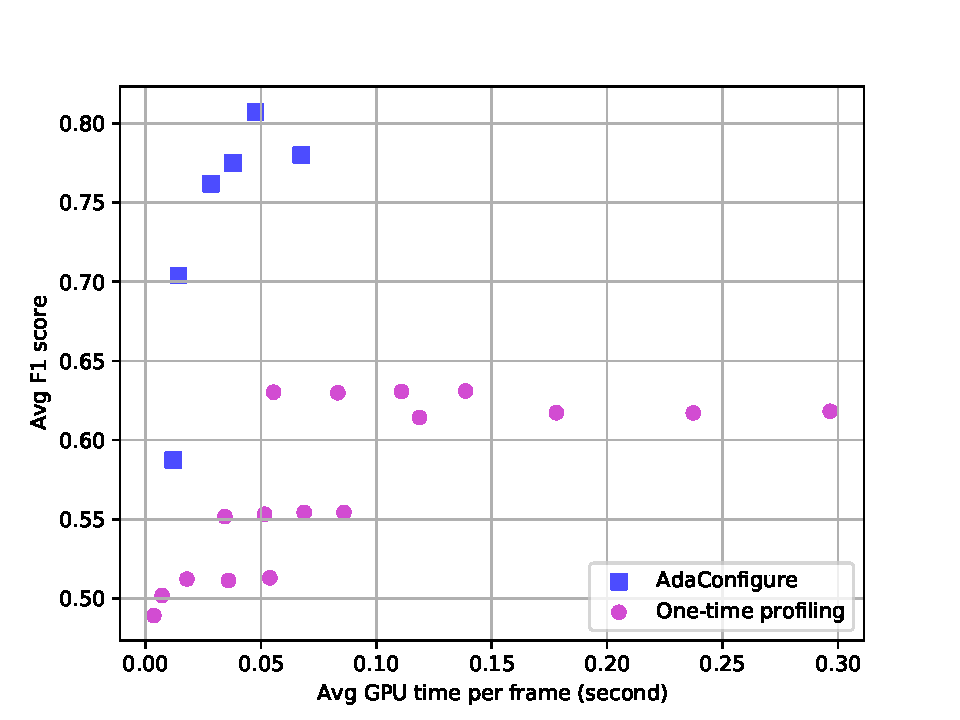
\includegraphics[width=5cm]{figures/Rear.pdf}}
%		\centerline{(c) Camera 3 }%(Bounding box-based)}
%		\centerline{(Bounding box-based)}
%	\end{minipage}		
%	\caption{AdaConfigure (blue) consistently outperforms the baseline of one-time profiling (magenta) across different cameras.}
%	\label{fig: 3dataset results}
%	%	\vspace{-0.5cm}
%\end{figure}
%
%To compare AdaConfigure's performance on single-camera inference and multi-camera inference, we respectively train and test the agent on each single-camera dataset of Multi-Camera Dataset. Figure \ref{fig: 3dataset results}(a)(b)(c) shows that AdaConfigure achieves 10-20\% higher accuracy with a similar amount of computation resources. 
%%or achieves similar accuracy with only 50-60\% of the computation resource on the single-camera inference. 
%As shown in Figure \ref{fig: results}(e), the gap between AdaConfigure and static configuration is larger than Figure \ref{fig: 3dataset results}(a)(b)(c), indicating that AdaConfigure has a better improvement on the multi-camera situation. AdaConfigure achieves 25-35\% higher accuracy with a similar amount of resources.
%%or reach higher accuracy with only 75-85\% of the resources on multi-camera inference.
%AdaConfigure achieves superior performance on multi-camera inference than single-camera inference. Instead of the static solution using fixed configuration in different situations, AdaConfigure can choose a proper configuration for different situations since the exact spatial characteristics of the video contents are different in different locations.


%It proves that our solution can pick the proper configuration according to intrusive dynamics of video contexts, including spatial and temporal features.

%\begin{figure*}[!t]
%	\begin{minipage}[t]{0.32\linewidth}
%		\centerline{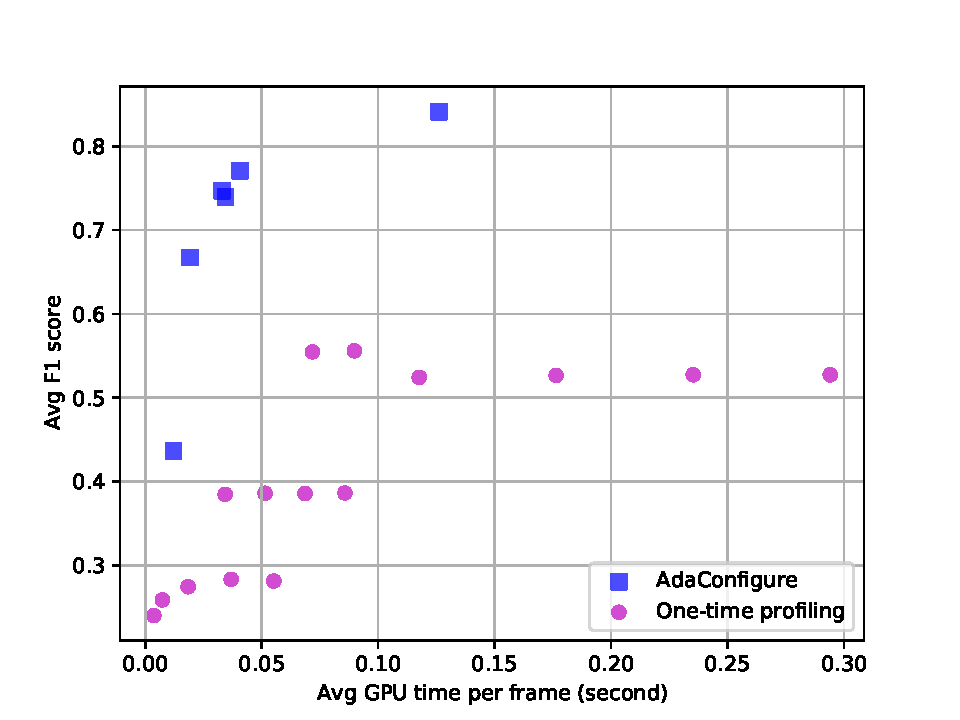
\includegraphics[width=6.5cm]{figures/Westbound.pdf}}
%		\centerline{(a) Camera 1 (Bounding box-based)}
%	\end{minipage}
%	\hfill
%	\begin{minipage}[t]{0.32\linewidth}
%		\centerline{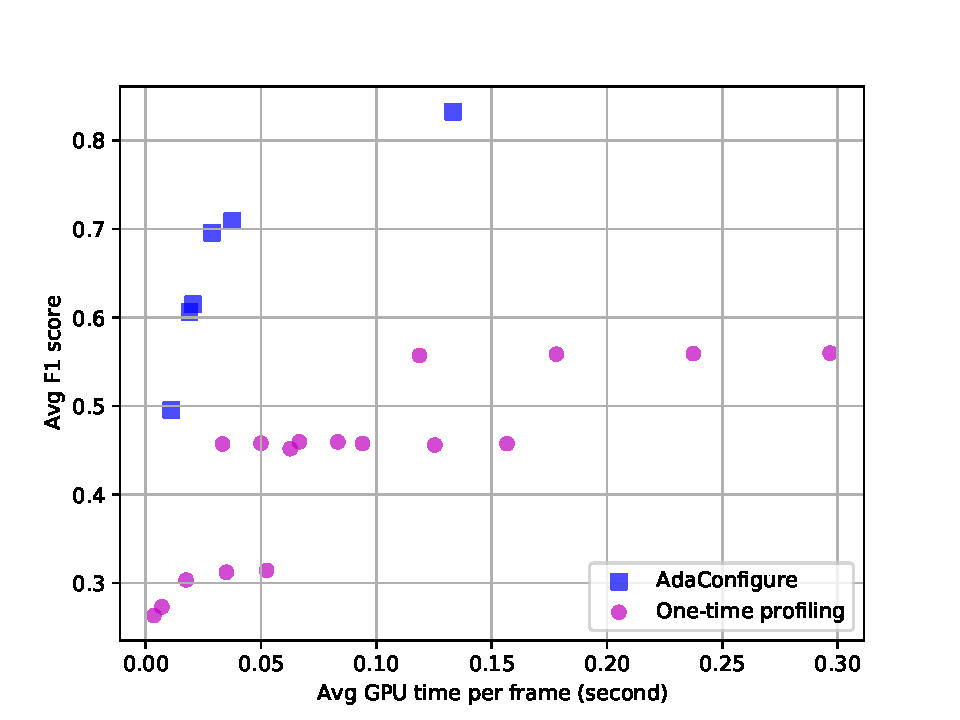
\includegraphics[width=6.5cm]{figures/Eastbound.pdf}}
%		\centerline{(b) Camera 2 (Bounding box-based)}
%	\end{minipage}
%	\hfill
%	\begin{minipage}[t]{0.32\linewidth}
%		\centerline{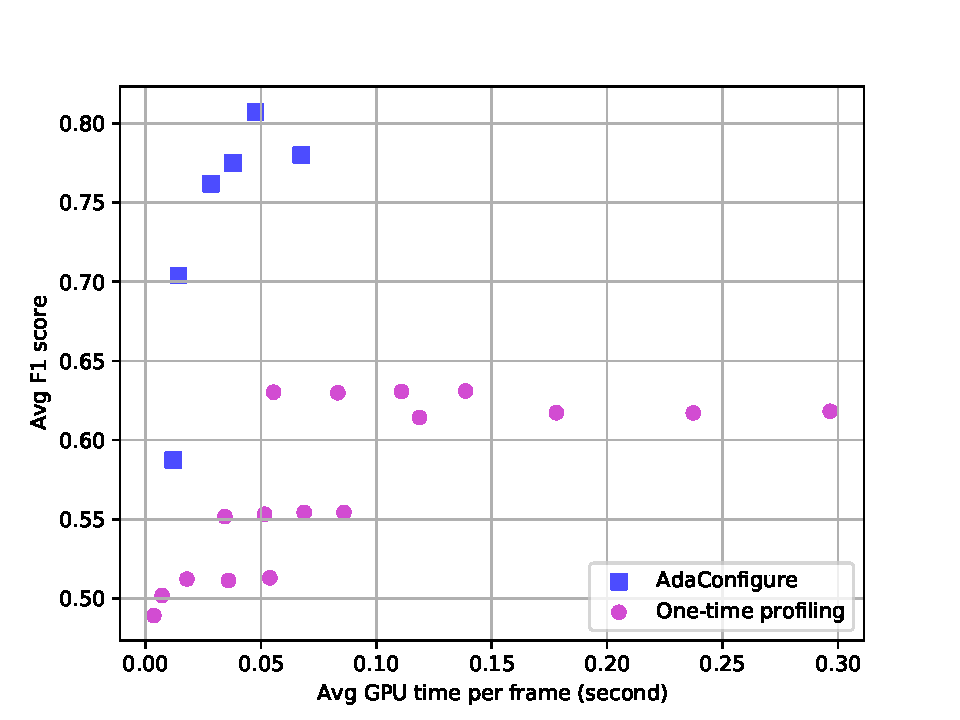
\includegraphics[width=6.5cm]{figures/Rear.pdf}}
%		\centerline{(c) Camera 3 (Bounding box-based)}
%	\end{minipage}		
%	\caption{AdaConfigure (blue) consistently outperforms the baseline of one-time profiling (magenta) across different cameras.}
%	\label{fig: 3dataset results}
%\end{figure*}
 
%\noindnet
 
\subsubsection{Low Profiling Cost of Adaptive Configuration}
\label{subsec: profiling cost}
%Comparing to the static solution that profiles configurations once, in our solution, the video
%chunk is passed to the AdaConfigure firstly to estimate the configuration. Running this RL agent brings profiling cost (extra resource consumption) to the whole system. 
%In this section, we evaluate this profiling cost. 
%In the inference phase, we divide the video into $T$-second intervals as video chunks and use AdaConfigure to choose the proper configuration for the first t seconds of the video chunk. It then sticks with the chosen configuration for the rest of the video chunk, i.e., for $T-t$ seconds. We use T = 4 and t = 1 for our experiments.
In our solution, the video chunk is passed to the AdaConfigure firstly to estimate the configuration, bringing profiling cost (extra resource consumption) to the whole system. 
The profiling cost, including the resource of extract $k_1$ embeddings and the cost of agent choosing actions. We test the average time on 30 hours video of Multi-Camera Dataset, and conclude that the average time of extract one embedding is 0.02s, and the average time of agent choosing action is 0.0006s, which can be ignored. We compute the ratio by dividing profiling time into total inference time as metric of profiling cost.
%, which is equals the frame number multiply the average time per frame. 
The profiling cost is about 0.2-2\% of the overall video analytics resource consumption. The concrete ratio depends on the concrete AdaConfigure configuration solutions, such as the solutions listed in Table \ref{tab: different sulutions}. For instance, when using the $\beta$ 0.7 solution, the profiling time is only 0.2\% of overall resource consumption on this solution; when using the $\beta$ 0.2 solution, the profiling cost is 1.5\%.        

\subsubsection{Different AdaConfigure Solutions to Meet Different Services}
\label{subsec: different sulutions}
In the training phase, when using different balance factors $\beta$ in the reward function, we would obtain different agents (different adaptive configuration strategies). 
%Each exact $\beta$ solution represents a concrete adaptive configuration strategy, which can adaptively update configuration across time. 
In general, the $\beta$ is bigger, indicating the accuracy is more important relatively, and the agent would choose a more expensive configuration. In our experiment, we set $\beta$ is 0.2,0.3,...,0.7, and the results of different AdaConfigure solutions on Multi-Camera Dataset are listed in Table \ref{tab: different sulutions}. 

\begin{table}[!t]
	\centering
	%     \begin{tabular}{lll}
	\resizebox{0.4\textwidth}{!}{
		\begin{tabular}{ccc}
			\toprule
			balance factor $\beta$ & Avg GPU time per frame (second) & Avg F1 score  \\ \midrule
			0.2          & 0.01384  &  0.64307            \\
			0.3          & 0.03314  &  0.72008            \\
			0.4          & 0.05203  &  0.79096            \\
			0.5          & 0.08479  &  0.80056            \\
			0.6          & 0.17570  &  0.87731            \\
			0.7          & 0.26511  &  0.93262            \\
			\bottomrule
	\end{tabular}}
	\caption{Resource consumption and bounding box-based F1 for different AdaConfigure solutions}
	\label{tab: different sulutions}
	%	\vspace{-0.1cm}
\end{table}

Table \ref{tab: different sulutions} shows that when the $\beta$ increases, the resource consumption and the accuracy of the corresponding solution would increase, indicating the AdaConfigure solutions of big $\beta$ would choose the more expensive configuration to inference. We can leverage this to train proper configuration strategy for different service demands, for example, using big $\beta$ for high-accuracy demand services and using small $\beta$ for low-accuracy demand services. 
%\begin{table}[!t]
%%\begin{table}[H]
%	\centering
%	%     \begin{tabular}{lll}
%	\resizebox{0.5\textwidth}{!}{
%		\begin{tabular}{lcc}
%			\toprule
%			Model and Image size & Inference time & Accuracy  \\ \midrule
%			SSD MobileNetV2 320p          & 49.5 ms  &  xxx            \\
%			SSD MobileNetV2 640p          & 58.5 ms  &  0.494            \\
%			SSD ResNet152V1 640p          & 100 ms  &  0.579            \\
%			SSD ResNet152V1 1024p          & 182.3 ms  &  0.614            \\
%			FasterRCNN ResNet50V1 640p          & 106.4 ms  &  0.637            \\
%			FasterRCNN ResNet50V1 1024p          & 120.5 ms  &  0.786           \\
%			FasterRCNN InceptionResNetV2 640p          & 361.8 ms  &  0.734            \\
%			FasterRCNN InceptionResNetV2 1024p          & 418.4 ms  &  1            \\
%			\bottomrule
%	\end{tabular}}
%	\caption{Inference time and F1 for different models and resolutions car truck}
%	\label{tab: latency-overhead}
%	% \vspace{-0.5cm}
%\end{table}
%
%\begin{table}[!t]
%	%\begin{table}[H]
%	\centering
%	%     \begin{tabular}{lll}
%	\resizebox{0.5\textwidth}{!}{
%		\begin{tabular}{lcc}
%			\toprule
%			Model and Image size & Inference time & Accuracy  \\ \midrule
%			SSD MobileNetV2 320p          & 49.5 ms  &  xxx            \\
%			SSD MobileNetV2 640p          & 58.5 ms  &  0.753            \\
%			SSD ResNet152V1 640p          & 100 ms  &  0.886            \\
%			SSD ResNet152V1 1024p          & 182.3 ms  &  0.942            \\
%			FasterRCNN ResNet50V1 640p          & 106.4 ms  &  0.889            \\
%			FasterRCNN ResNet50V1 1024p          & 120.5 ms  &  0.98           \\
%			FasterRCNN InceptionResNetV2 640p          & 361.8 ms  &  0.965            \\
%			FasterRCNN InceptionResNetV2 1024p          & 418.4 ms  &  1            \\
%			\bottomrule
%	\end{tabular}}
%	\caption{Inference time and F1 for different models and resolutions}
%	\label{tab: latency-overhead}
%	% \vspace{-0.5cm}
%\end{table}

%\begin{figure}[!t]
%	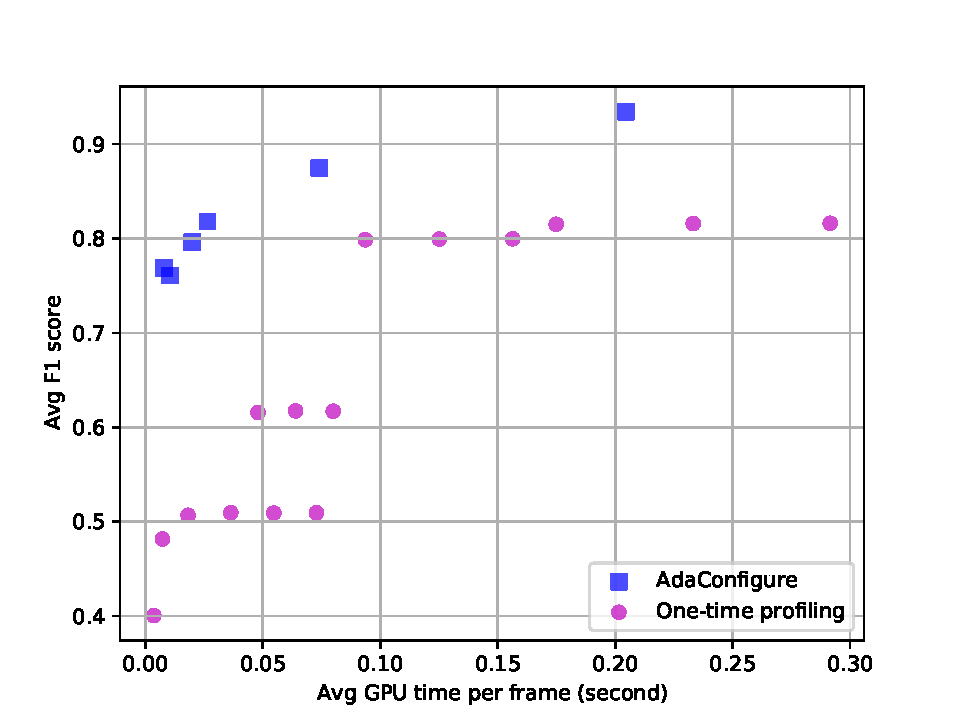
\includegraphics[width=9cm,height=8cm]{figures/m6.pdf}
%	\centering
%	\caption{The effect of different models, frame rate, and resolutions on accuracy and processing time. AdaConfigure (blue) consistently outperforms the baseline of one-time update (magenta) across different datasets. Each dot represents the results of running each solution.}
%	\label{fig_m6}
%\end{figure}